

\newpage
\begin{figure}[h]
	\makebox[\textwidth]{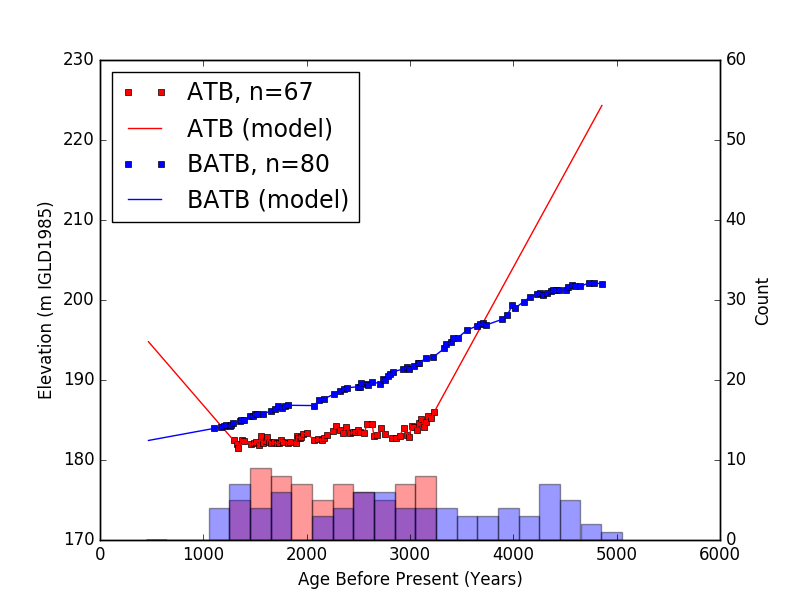
\includegraphics[width=0.72\paperwidth]{data/ATB-BATB_DataAndModel.png}}
	\caption{ATB-BATB raw data with linear interpolation model}
	\label{fig:data_ATBxBATB}
\end{figure}
The data available for sites ATB and BATB shows two of the most common trends in
 the data used in this paper; Data is available for both sites from
 approximately 1000 years before present to roughly 3300 years before present,
 with a gap in the record at around 2000 years before present (caused by a low
 water level period preferentially not forming beach deposits during this time)
 (Johnston et al, 2014). The regressions derived from this pair of data sets,
 seen in Figures \ref{fig:gias_ATBxBATB} \& \ref{fig:gias_BATBxATB}, are well
 constrained, and produce a moderately well constrained value on relative GIA
 between ATB and BATB of 25-30 cm/century. A plot of the confidence intervals
 for the slopes obtained from each linear regression can be seen in Figure \ref{fig:intervalsGIA}


\newpage

\begin{figure}[h]
	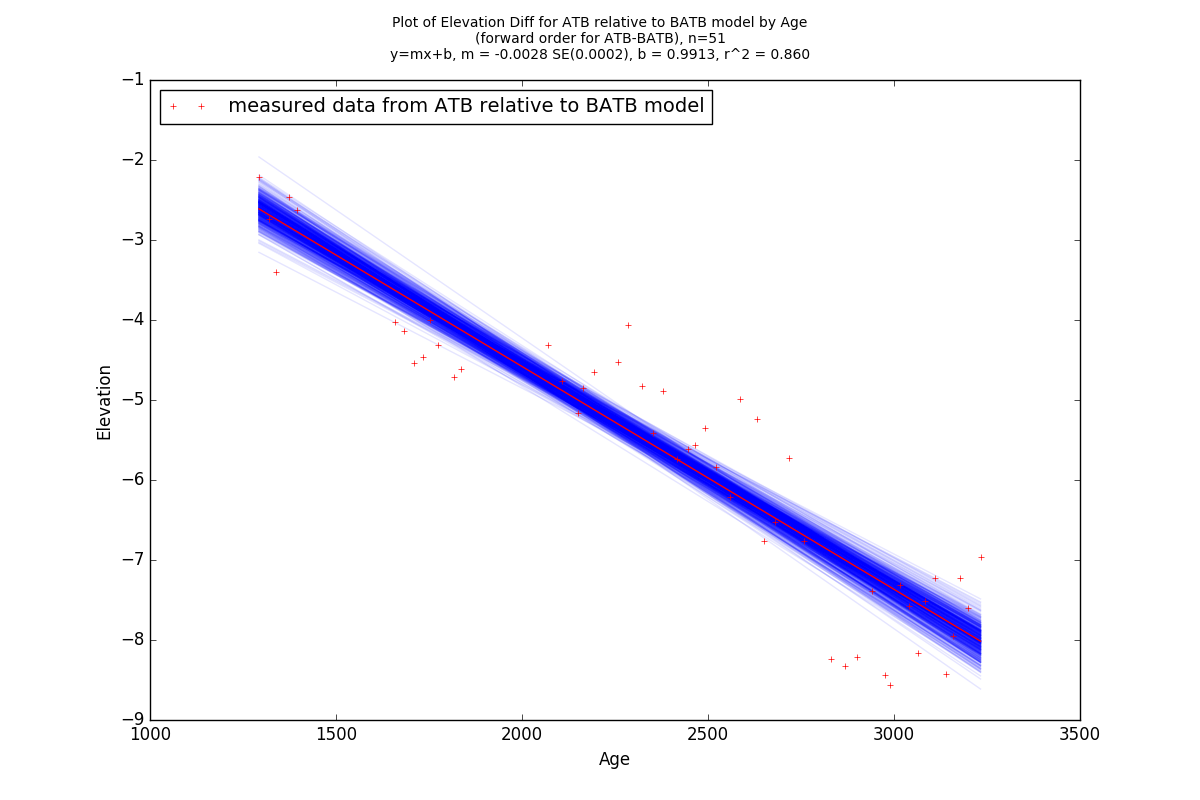
\includegraphics[width=0.9\linewidth]{data/bothNonZero/withinSeventyFivePercent/gias/theGIA_ATB_relative_to_BATB.png}
	\caption{Differences in elevation measured from the ATB data to the ATB model}
	\label{fig:gias_ATBxBATB}
\end{figure}
\newpage


\begin{figure}[h]
	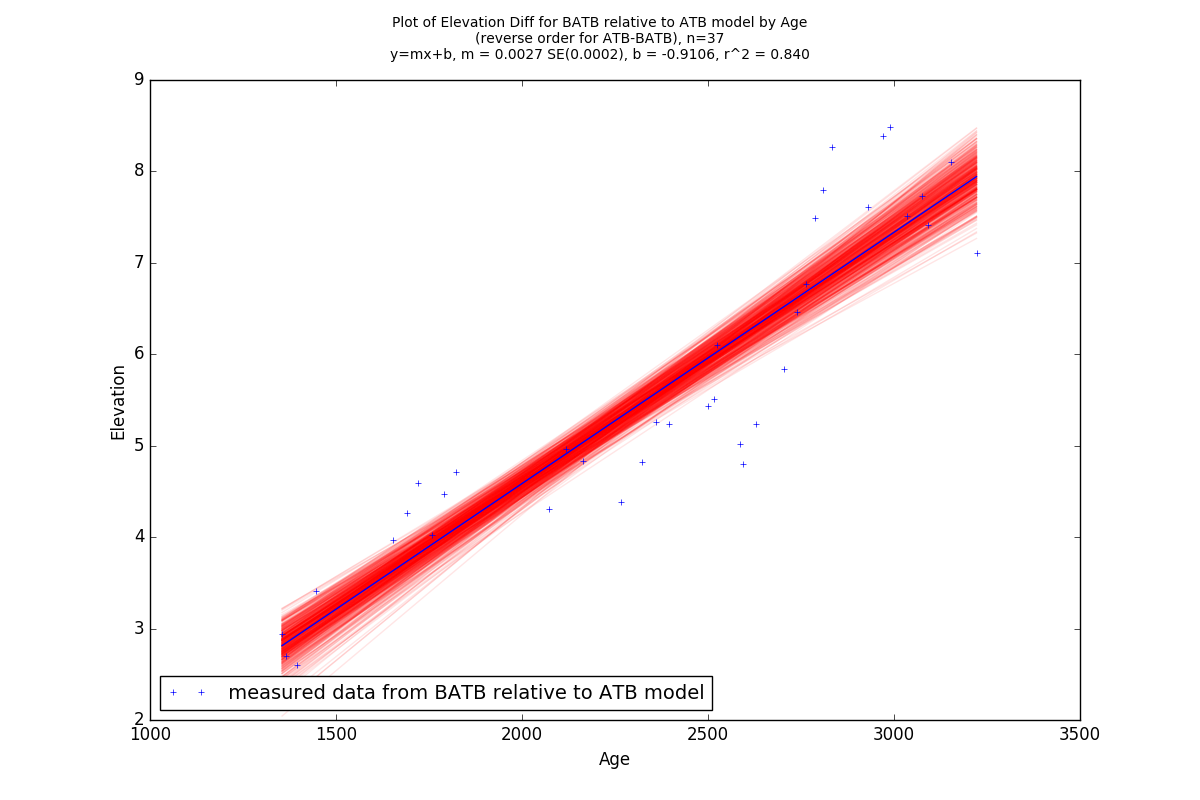
\includegraphics[width=0.9\linewidth]{data/bothNonZero/withinSeventyFivePercent/gias/theGIA_BATB_relative_to_ATB.png}
	\caption{Differences in elevation measured from the BATB data to the ATB model}
	\label{fig:gias_BATBxATB}
\end{figure}
\newpage
% this desperately needs to be done as a loop



\begin{figure}[h]
	\makebox[\textwidth]{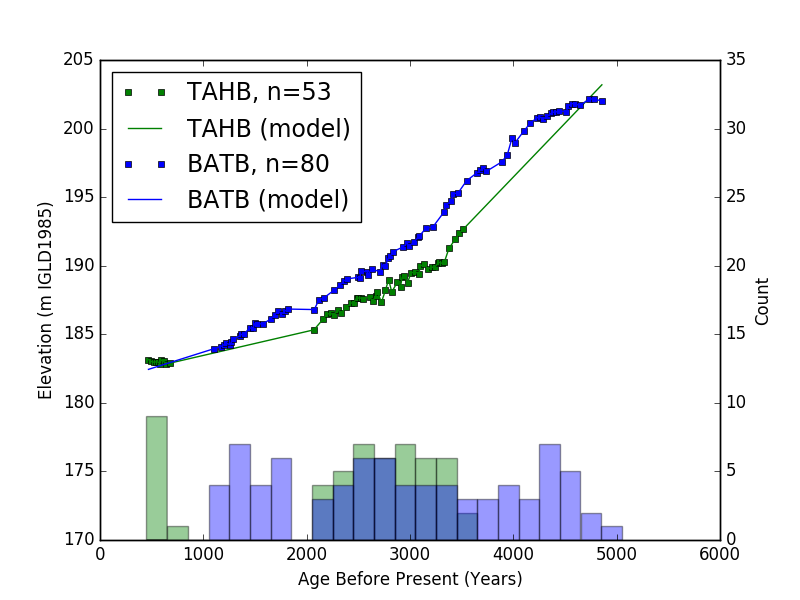
\includegraphics[width=0.72\paperwidth]{data/TAHB-BATB_DataAndModel.png}}
	\caption{TAHB-BATB raw data with linear interpolation model}
	\label{fig:data_TAHBxBATB}
\end{figure}

The data plot for the site combination of TAHB and BATB shows a common issue
with comparing datasets, as the data with ages more recent than the 2000 year before
present gap is unsable. This is because the regions where data is available for
one dataset are empty of datapoints for the other, making the modelled prediction
of the other dataset highly unreliable. As a result, a filter is applied to the
data to prevent this, grouping data points into bins 200 years wide, and
ignoring the data points from bins in which either data set had no datapoints,
as well as any which had bin counts differing by more than 75\% for that bin.
The linear regressions produced from this dataset seen in Figures 
\ref{fig:gias_TAHBxBATB} \& \ref{fig:gias_BATBxTAHB}, are well constrained, and
report a value for relative GIA of between 12-16 cm/century.

\newpage

\begin{figure}[h]
	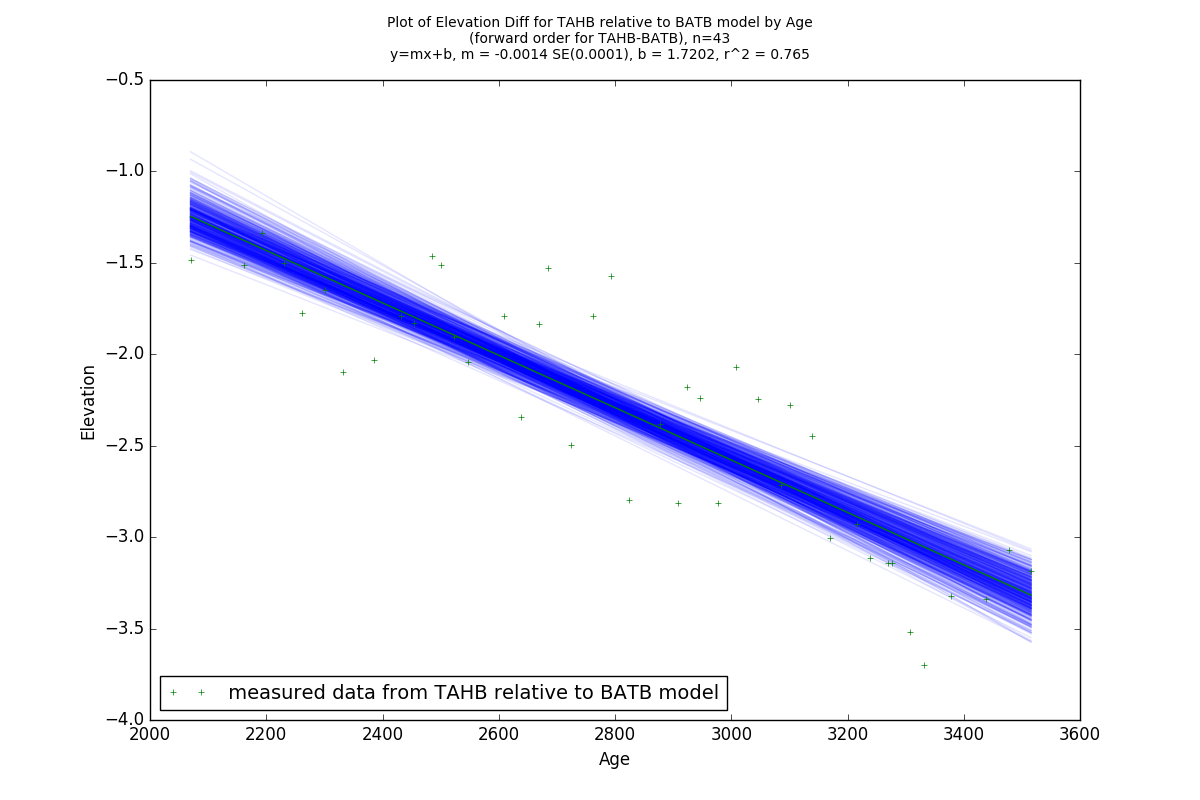
\includegraphics[width=0.9\linewidth]{data/bothNonZero/withinSeventyFivePercent/gias/theGIA_TAHB_relative_to_BATB.png}
	\caption{Differences in elevation measured from the TAHB data to the BATB model}
	\label{fig:gias_TAHBxBATB}
\end{figure}
\newpage


\begin{figure}[h]
	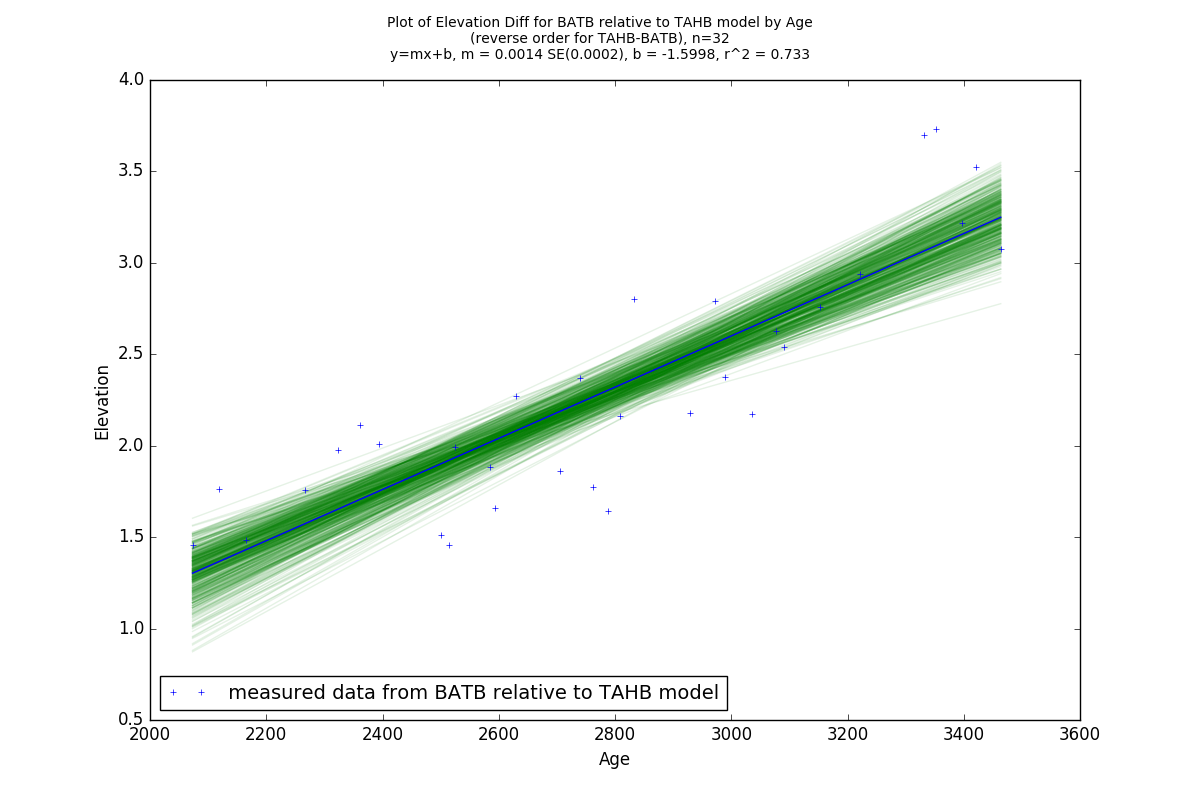
\includegraphics[width=0.9\linewidth]{data/bothNonZero/withinSeventyFivePercent/gias/theGIA_BATB_relative_to_TAHB.png}
	\caption{Differences in elevation measured from the BATB data to the TAHB model}
	\label{fig:gias_BATBxTAHB}
\end{figure}
\newpage








\begin{figure}[h]
	\makebox[\textwidth]{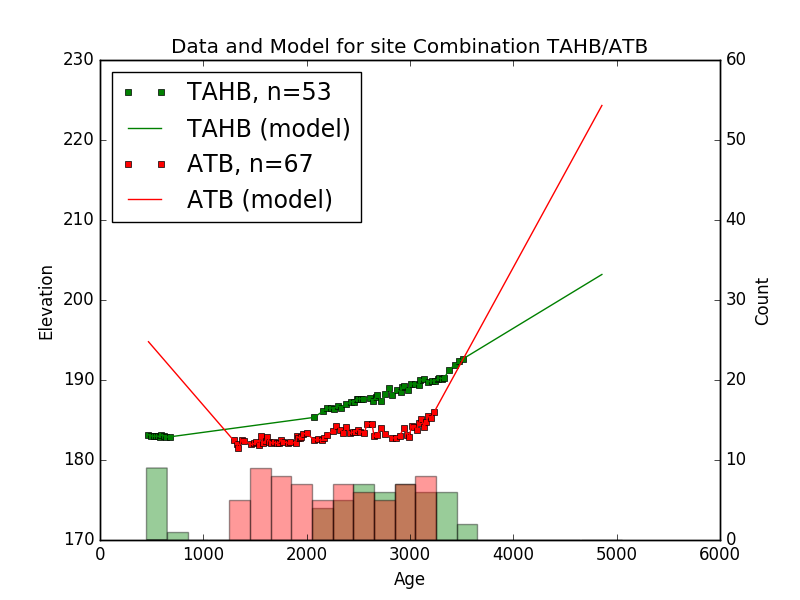
\includegraphics[width=0.72\paperwidth]{data/TAHB-ATB_DataAndModel.png}}
	\caption{TAHB-ATB raw data with linear interpolation model}
	\label{fig:data_TAHBxATB}
\end{figure}

Similarly the combination of TAHB and ATB are constrained to ages older than
2000 years before present, but also have a much shorter range of age values that
can be considered for GIA calculation, ending at around 3100 years before present.
This results in regressions that are not as well constrained, giving a value for
relative GIA of between 20-29 cm/century.

\newpage

\begin{figure}[h]
	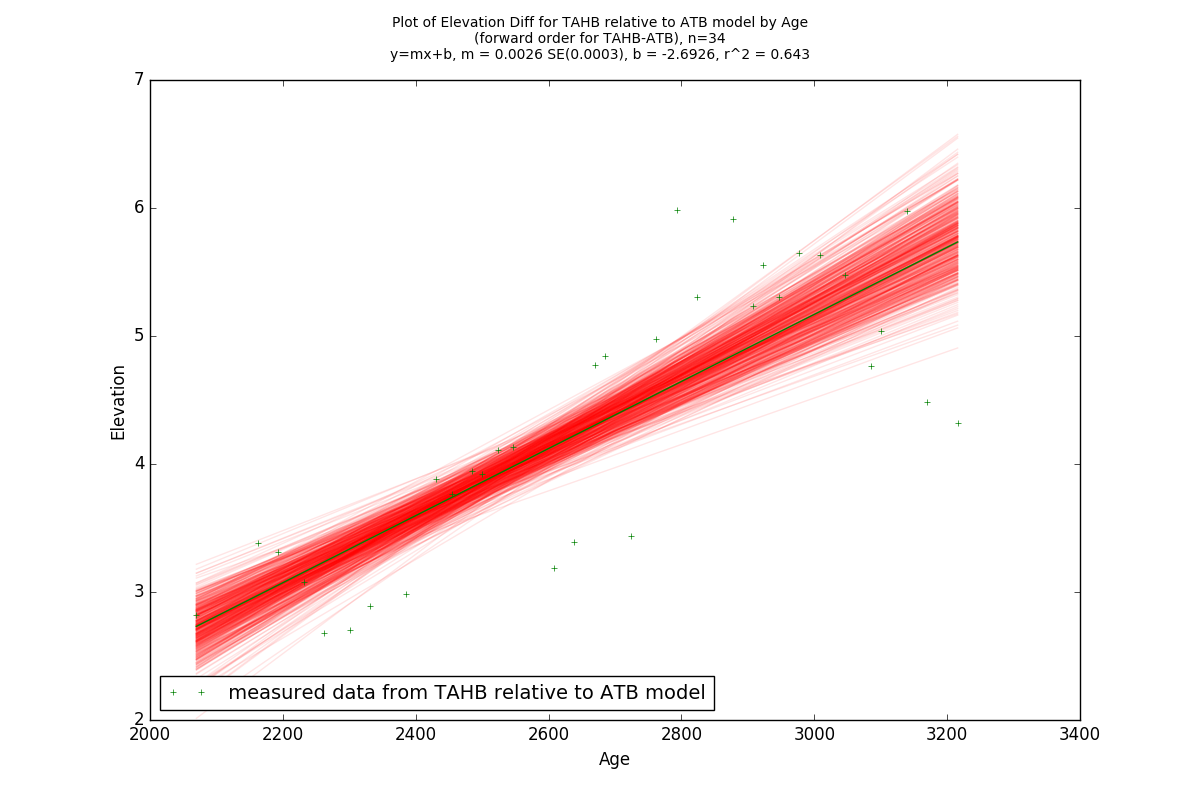
\includegraphics[width=0.9\linewidth]{data/bothNonZero/withinSeventyFivePercent/gias/theGIA_TAHB_relative_to_ATB.png}
	\caption{Differences in elevation measured from the TAHB data to the ATB model}
	\label{fig:gias_TAHBxATB}
\end{figure}
\newpage


\begin{figure}[h]
	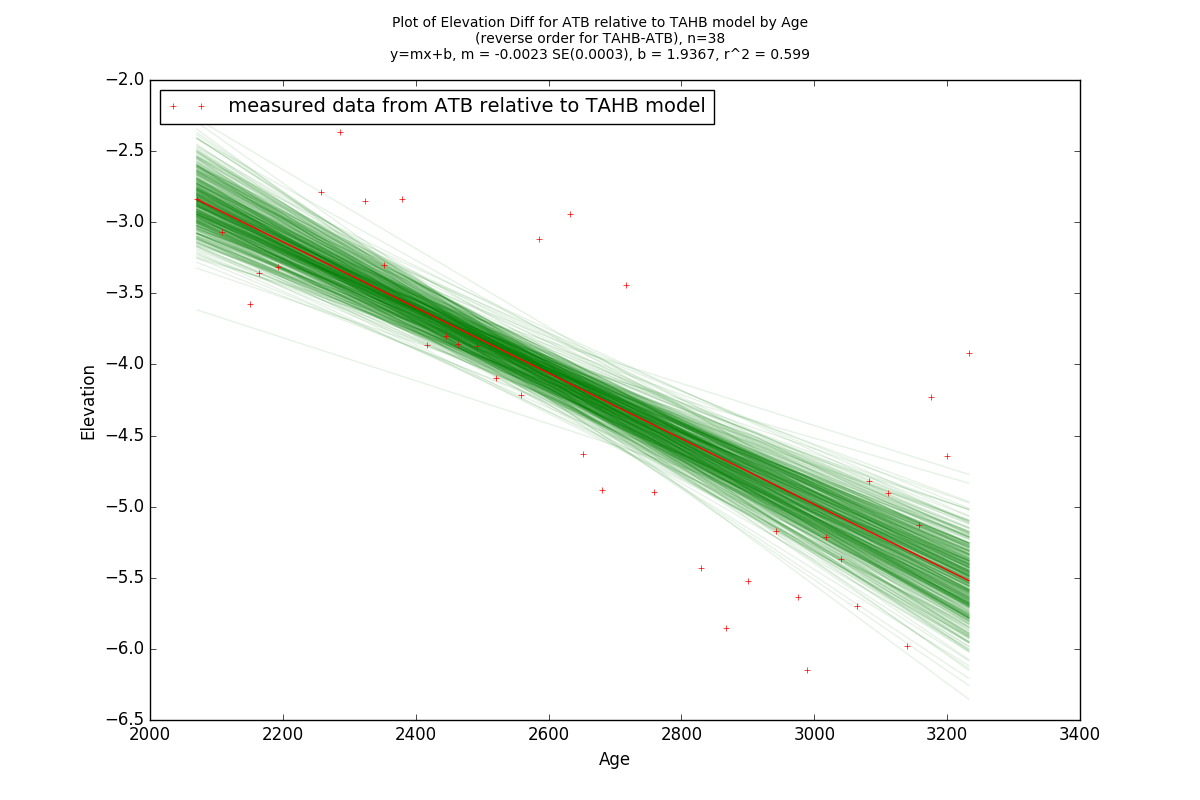
\includegraphics[width=0.9\linewidth]{data/bothNonZero/withinSeventyFivePercent/gias/theGIA_ATB_relative_to_TAHB.png}
	\caption{Differences in elevation measured from the ATB data to the TAHB model}
	\label{fig:gias_ATBxTAHB}
\end{figure}
\newpage






\begin{figure}[h]
	\makebox[\textwidth]{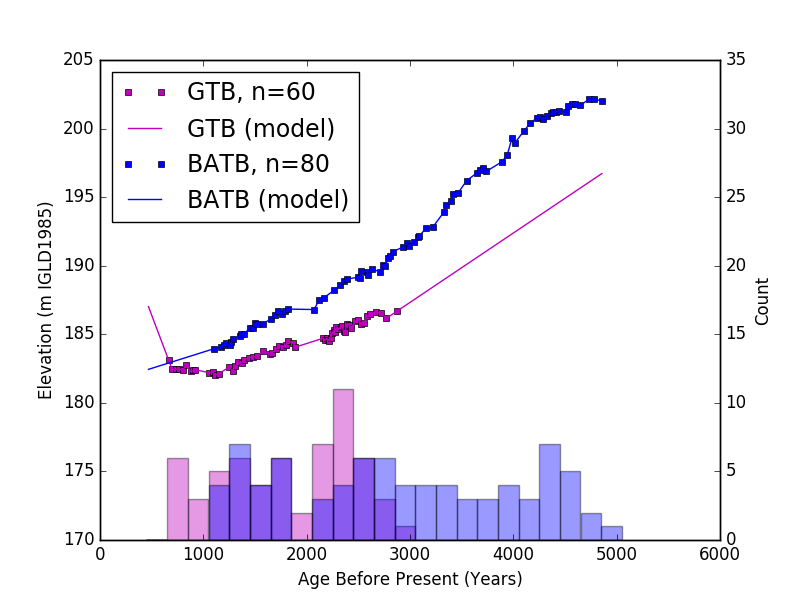
\includegraphics[width=0.72\paperwidth]{data/GTB-BATB_DataAndModel.png}}
	\caption{GTB-BATB raw data with linear interpolation model}
	\label{fig:data_GTBxBATB}
\end{figure}
The GTB BATB combination has a data spread similar to that of ATB \& BATB, albeit
with a data range slightly shifted towards the present day. The regressions in
Figures \ref{fig:gias_GTBxBATB} \& \ref{fig:gias_BATBxGTB} bear this out,
producing one of the better constrained values at 11-13 cm/century.
\newpage

\begin{figure}[h]
	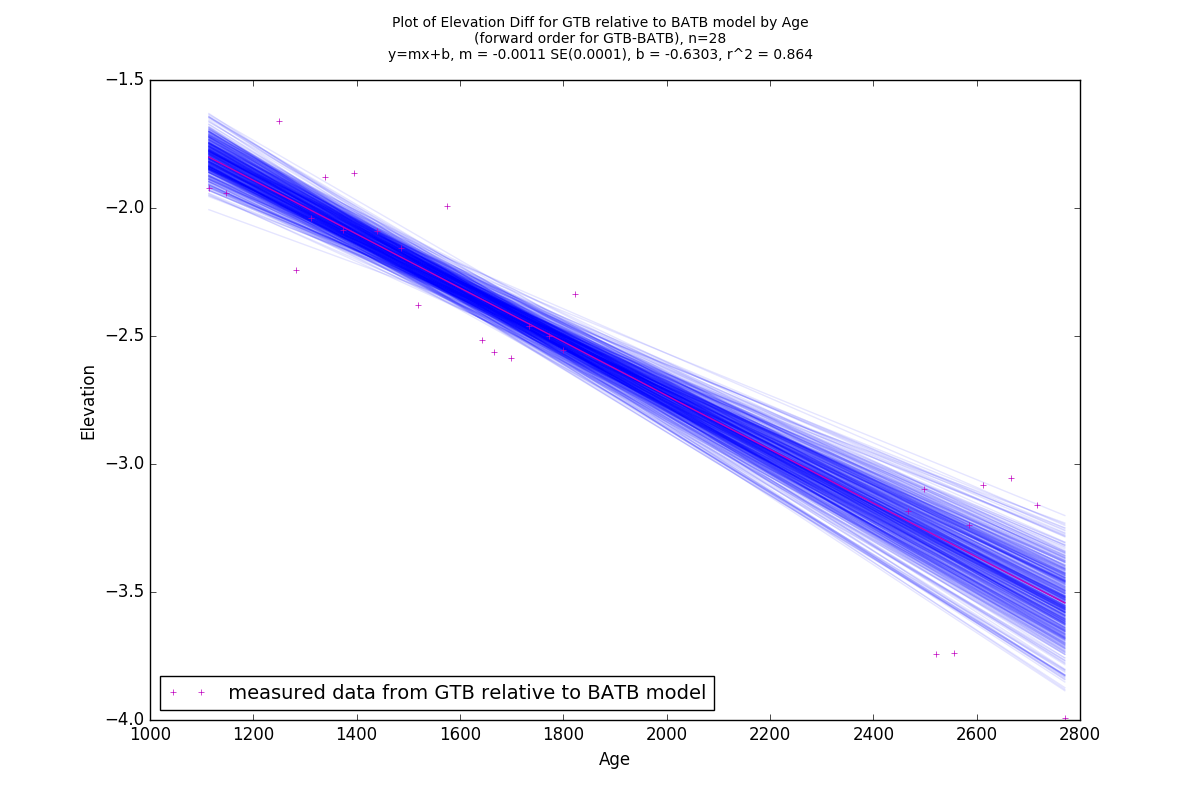
\includegraphics[width=0.9\linewidth]{data/bothNonZero/withinSeventyFivePercent/gias/theGIA_GTB_relative_to_BATB.png}
	\caption{Differences in elevation measured from the GTB data to the BATB model}
	\label{fig:gias_GTBxBATB}
\end{figure}
\newpage


\begin{figure}[h]
	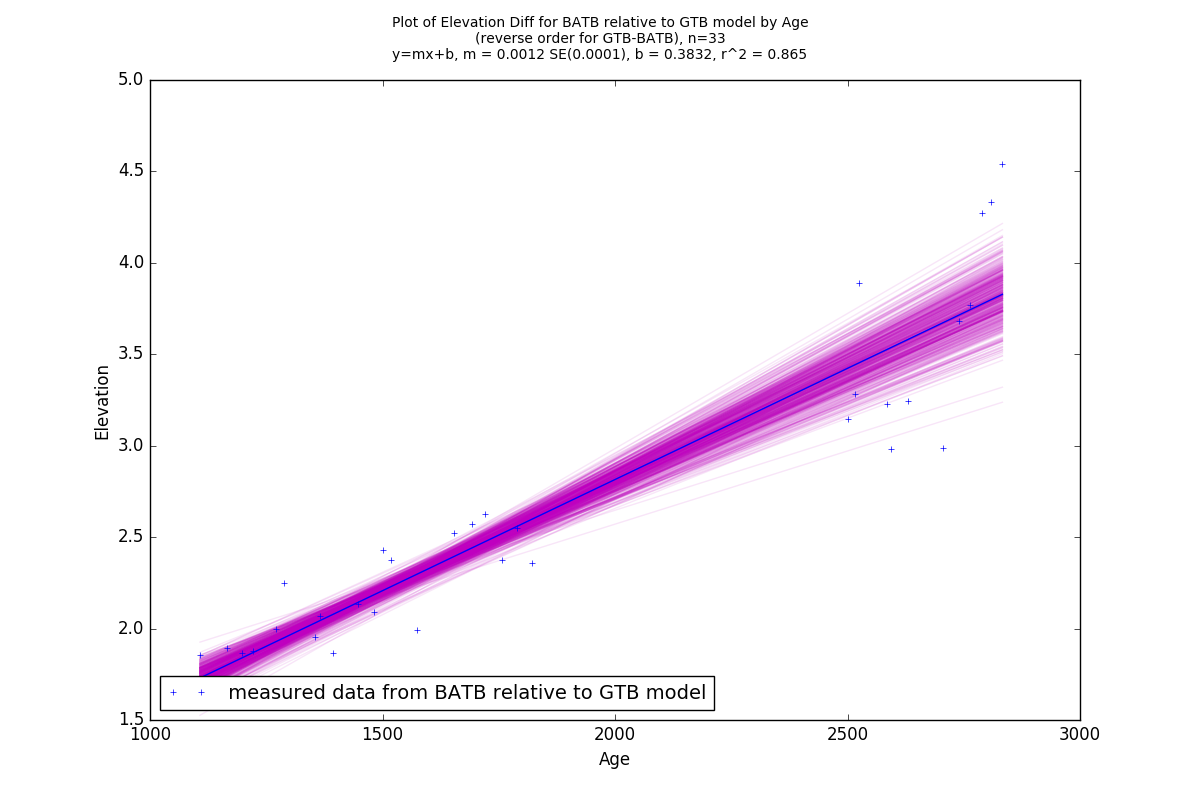
\includegraphics[width=0.9\linewidth]{data/bothNonZero/withinSeventyFivePercent/gias/theGIA_BATB_relative_to_GTB.png}
	\caption{Differences in elevation measured from the BATB data to the GTB model}
	\label{fig:gias_BATBxGTB}
\end{figure}
\newpage









\begin{figure}[h]
	\makebox[\textwidth]{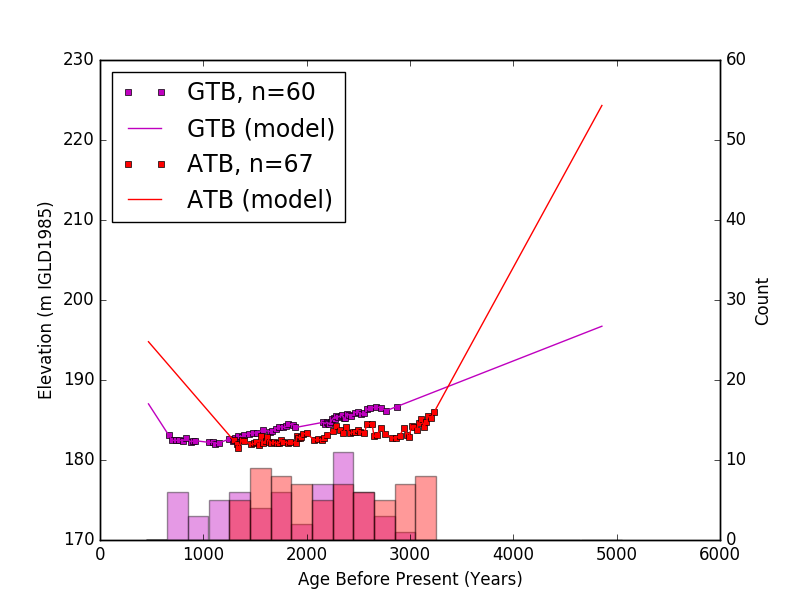
\includegraphics[width=0.72\paperwidth]{data/GTB-ATB_DataAndModel.png}}
	\caption{GTB-ATB raw data with linear interpolation model}
	\label{fig:data_GTBxATB}
\end{figure}

The GTB ATB combination is similar to most of the combinations looked at so far,
save for the fact that it has enough data available at the 2000 year before 
present gap to qualify for use under the filter. In spite of this, the
regressions in Figures \ref{fig:gias_GTBxATB} \& \ref{fig:gias_ATBxGTB} are
somewhat poorly constrained, giving a rate of GIA of 9-14 cm/century.
\newpage

\begin{figure}[h]
	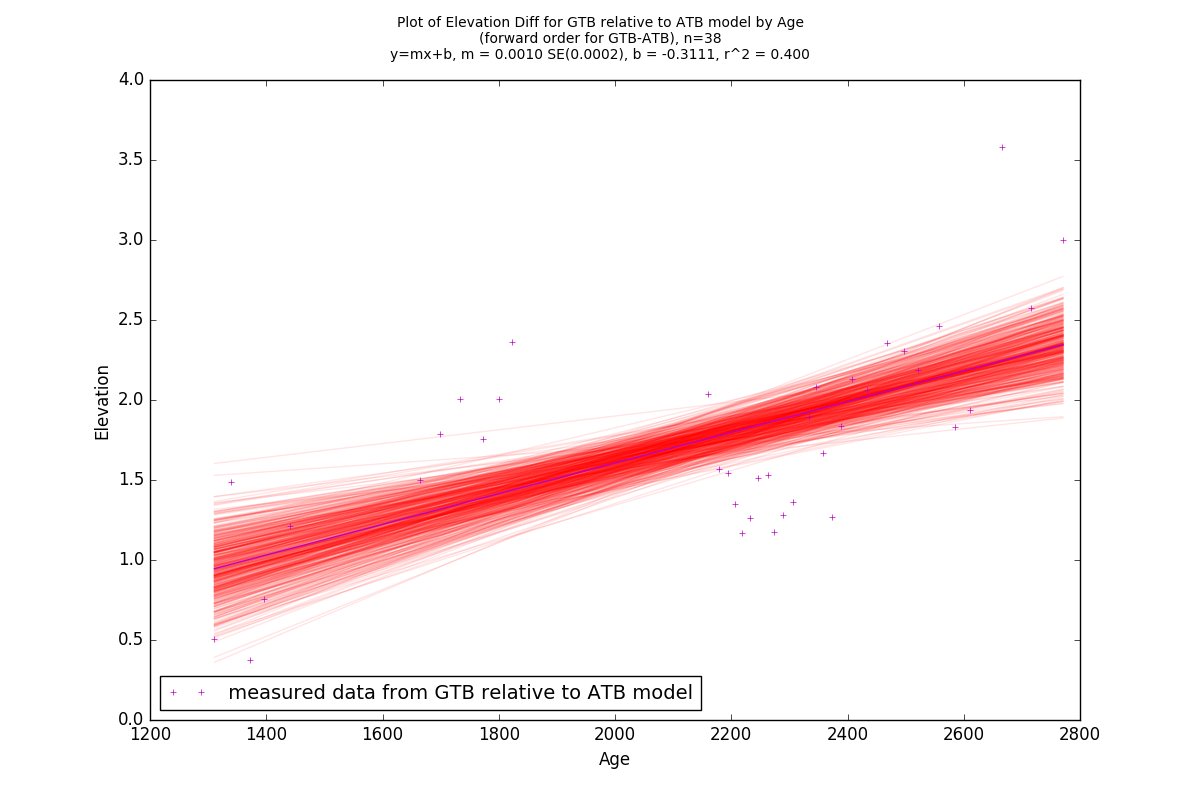
\includegraphics[width=0.9\linewidth]{data/bothNonZero/withinSeventyFivePercent/gias/theGIA_GTB_relative_to_ATB.png}
	\caption{Differences in elevation measured from the GTB data to the ATB model}
	\label{fig:gias_GTBxATB}
\end{figure}
\newpage


\begin{figure}[h]
	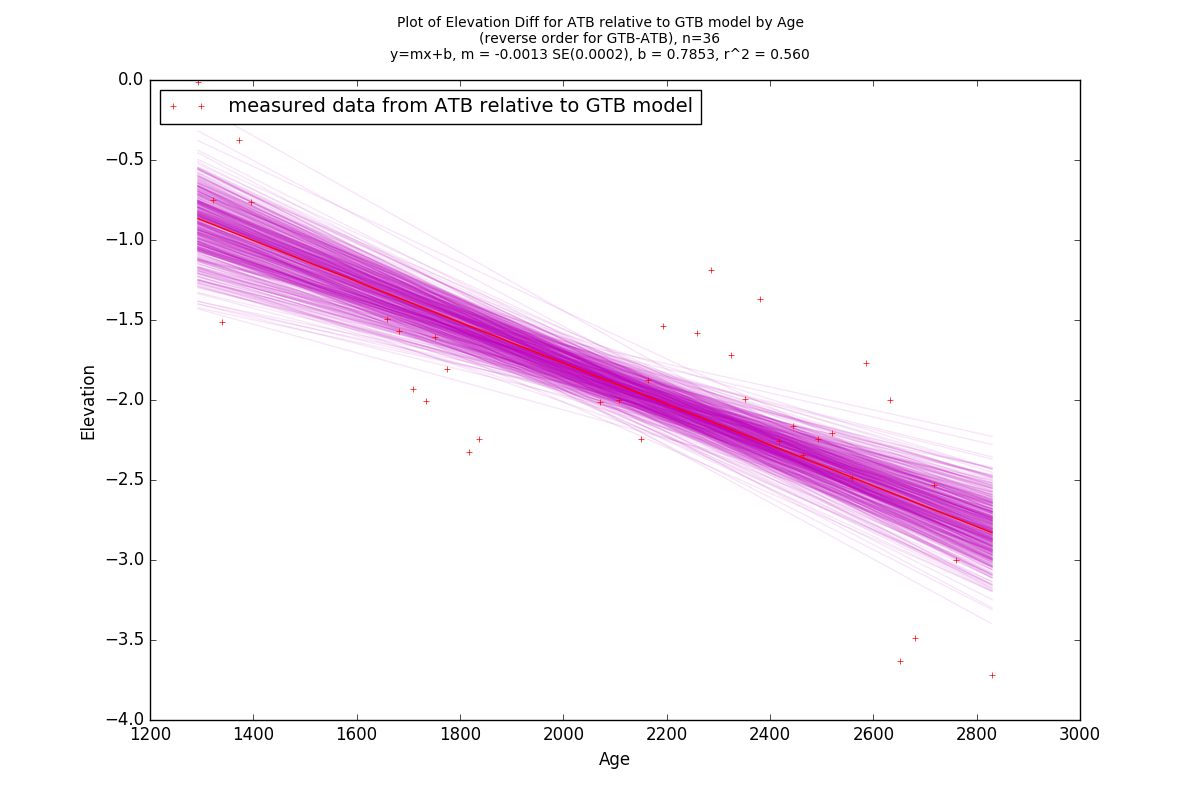
\includegraphics[width=0.9\linewidth]{data/bothNonZero/withinSeventyFivePercent/gias/theGIA_ATB_relative_to_GTB.png}
	\caption{Differences in elevation measured from the ATB data to the GTB model}
	\label{fig:gias_ATBxGTB}
\end{figure}
\newpage










\begin{figure}[h]
	\makebox[\textwidth]{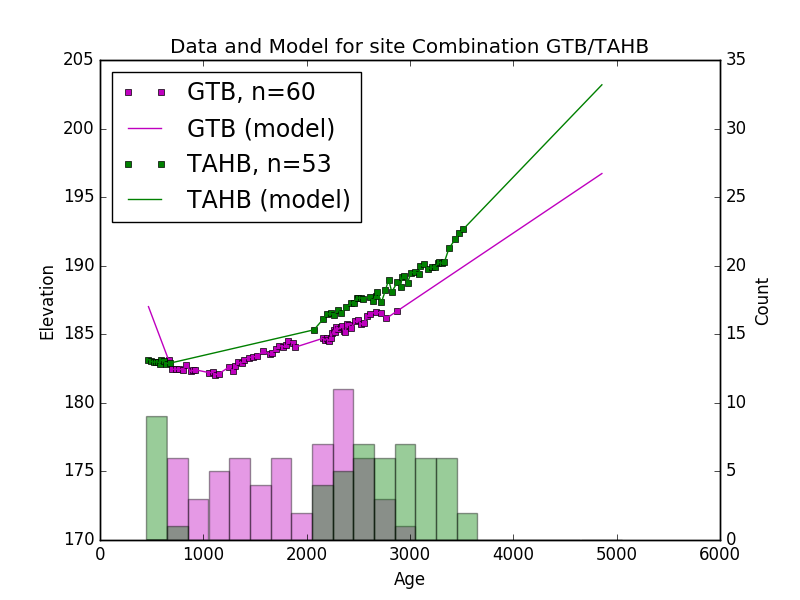
\includegraphics[width=0.72\paperwidth]{data/GTB-TAHB_DataAndModel.png}}
	\caption{GTB-TAHB raw data with linear interpolation model}
	\label{fig:data_GTBxTAHB}
\end{figure}
The final pair of sites GTB and TAHB has by far the most poorly constrained set
of regressions, likely due to the alignment of most of both datasets only giving
sample sizes of n=22 (Figure \ref{fig:gias_TAHBxGTB}) and n=27 (Figure \ref{fig:gias_GTBxTAHB}).
This resulted in an estimate of GIA that ranges anywhere from 3-8 cm/century.
\newpage

\begin{figure}[h]
	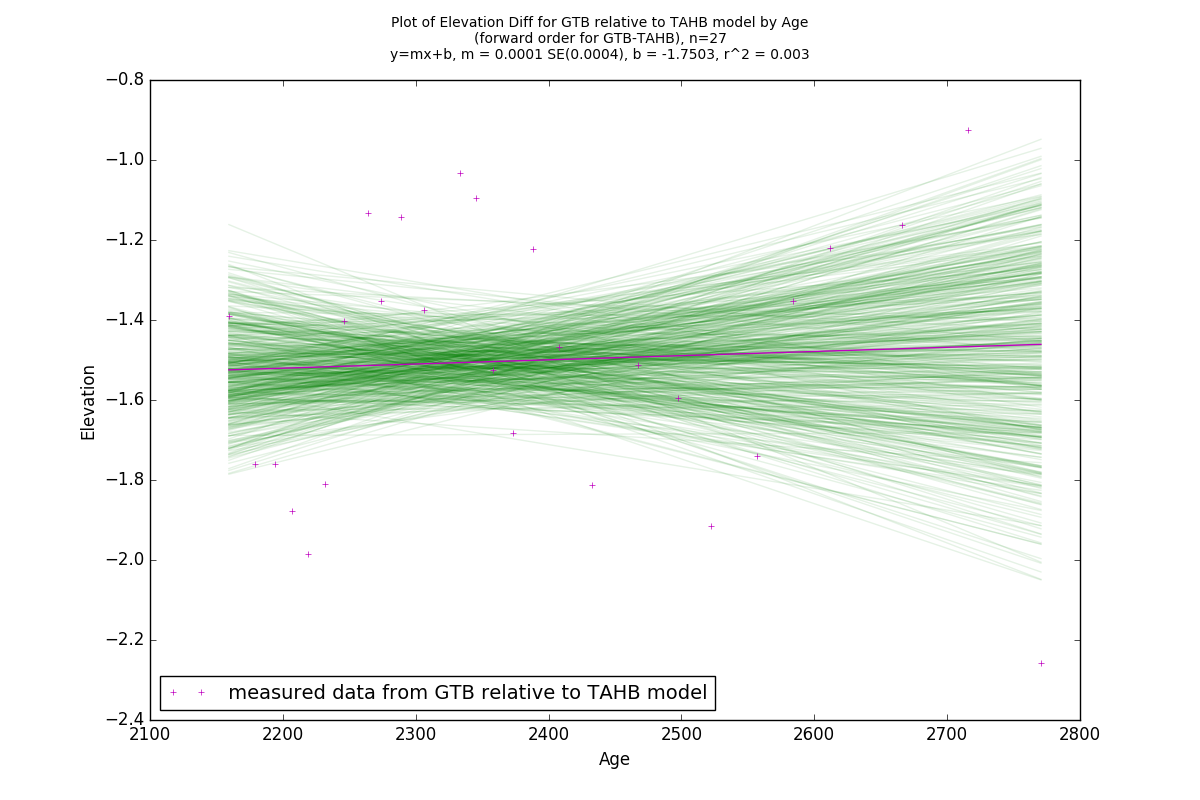
\includegraphics[width=0.9\linewidth]{data/bothNonZero/withinSeventyFivePercent/gias/theGIA_GTB_relative_to_TAHB.png}
	\caption{Differences in elevation measured from the GTB data to the TAHB model}
	\label{fig:gias_GTBxTAHB}
\end{figure}
\newpage


\begin{figure}[h]
	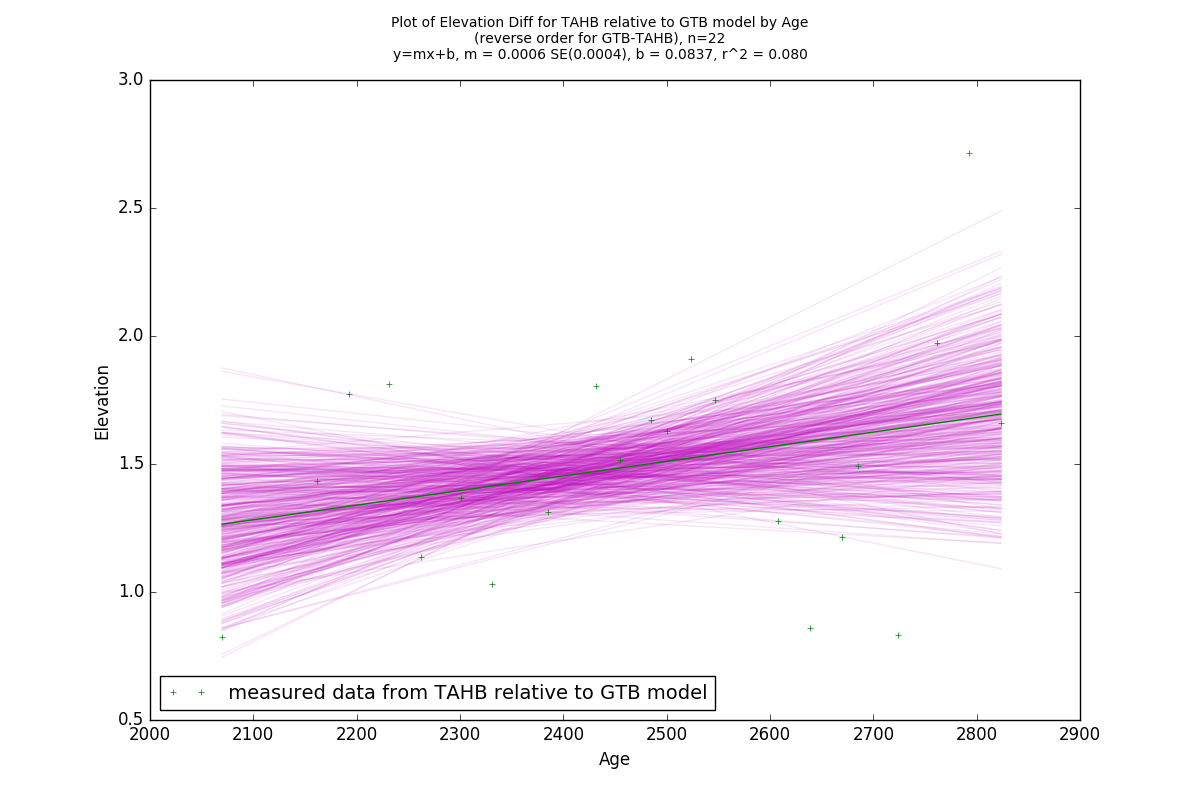
\includegraphics[width=0.9\linewidth]{data/bothNonZero/withinSeventyFivePercent/gias/theGIA_TAHB_relative_to_GTB.png}
	\caption{Differences in elevation measured from the TAHB data to the GTB model}
	\label{fig:gias_TAHBxGTB}
\end{figure}
\newpage


\begin{figure}[h]
	\makebox[\textwidth]{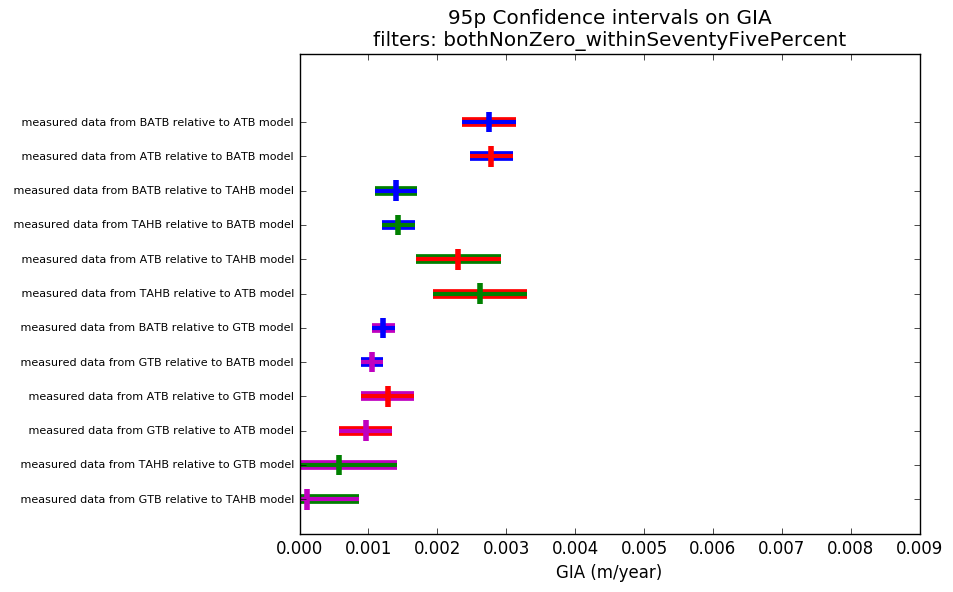
\includegraphics[width=0.6\paperwidth]{data/bothNonZero/withinSeventyFivePercent/gias/intervals.png}}
	\caption{95p Confidence intervals on GIA rates obtained from site comparisons}
	\label{fig:intervalsGIA}
\end{figure}


\newpage

